% !TeX encoding = utf-8
\documentclass[a4paper,12pt]{diplom}
\inputencoding{utf8}
\usepackage{paratype}
\DeclareMathSizes{12}{13.4}{11}{10}

\usepackage[left=3cm,right=2cm,top=2cm,bottom=2cm]{geometry} % Размеры полей
\usepackage[onehalfspacing]{setspace} % Полуторный интервал
%\renewcommand{\baselinestretch}{1.25} % Полуторный интервал
\usepackage{indentfirst} % Абзацный отступ в начале разделов
\setlength{\parindent}{1.25cm} % Величина абзацного отступа

\usepackage[pdftex]{graphicx} % Для вставки изображений
\usepackage{array} % Для таблиц
\usepackage{booktabs} % Для красивых таблиц 
\usepackage{tikz} % Рисунки с помощью TikZ
\usepackage[linesnumbered,lined,ruled]{algorithm2e} % Для оформления псевдокода
%\usepackage{algorithm} % Альтернатива оформления псевдокода
%\usepackage{algpseudocode} % Альтернатива оформления псевдокода
\usepackage{listings} % Оформление листингов программ
\usepackage{icomma} % Удаляем тонкий пробел после запятой в мат. режиме

% Если на нумерованную формулу нет ссылки в тексте,
\mathtoolsset{showonlyrefs} % то она становится ненумерованной

% microtype улучшает распределение символов в строке
\usepackage{microtype}  % Можно отключить, если возникают ошибки компиляции

% Формируем PDF с полноценными перекрестными ссылками
\usepackage[unicode, pdfborder={0 0 0}, pdfstartview=FitV]{hyperref}

% Часто используемые макросы
\newcommand{\N}{\mathbb{N}}  % Множество натуральных чисел
\newcommand{\Z}{\mathbb{Z}}  % Множество целых чисел
\newcommand{\R}{\mathbb{R}}  % Множество действительных чисел
\DeclareMathOperator{\sgn}{sgn} % Знак числа
\DeclareMathOperator{\M}{\mathsf{M}} % Матожидание
\newcommand{\from}{\colon} % Двоеточие в определении функции. Пример: $f \from \R \to \N$.
% Заменяем англоязычные обозначения на русские
\renewcommand{\le}{\leqslant}
\renewcommand{\leq}{\leqslant}
\renewcommand{\ge}{\geqslant}
\renewcommand{\geq}{\geqslant}
\renewcommand{\emptyset}{\varnothing}
\renewcommand{\epsilon}{\varepsilon}

%%%%%%%%%%%%%%%%%%%%%%%%%%
% Конец преамбулы
%%%%%%%%%%%%%%%%%%%%%%%%%%

\begin{document}

% Содержимое титульного листа

%\LetterHead{Минобр...}
\Kafedra{Кафедра информационных и сетевых технологий}

% Зав. кафедрой
\ZavKaf{Заведующий кафедрой,\\ к.\,ф.-м.\,н.}{Д.\,Ю.~Чалый}
% Если это курсовая работа и виза зав. каф. не нужна, раскомментируйте следующую строку
%\Kursovaya

% Вид работы: Курсовая работа, Выпускная квалификационная работа, 
\DocumentType{\large Выпускная квалификационная работа}

% Название дипломной работы
%\Title{\begin{Large}\bfseries Название дипломной работы\\ не помещающееся в одну строку\end{Large}}
\Title{\Large\bfseries Разработка клиентской части системы для автоматизации процесса рекрутирования сотрудников}

% Направление подготовки
\Napr{по направлению\\ 09.03.03 Прикладная информатика}

% Руководитель
\Chief{Научный руководитель\\ стар. преподаватель}{Н.\,В.~Легков}

% Автор
\Author{Студент группы ПИЭ-41БО}{О.\,С.~Гаршина}

%\City{Ярославль}
%\Year{2019}

% Создаем титульный лист
\maketitle

\chapter*{Реферат}

Объем \total{page} с., \total{chapternum} гл., \total{fignum} рис.,
\total{tablenum} табл., \total{bibnum} источников, \total{appnum} прил.

\medskip

Ключевые слова и выражения: \textbf{react, рекрутер, автоматизация, HR, резюме, front-end, JavaScript}

\medskip

Целью данной работы является разработка клиентской части приложения - HR-CV Portal, который оптимизирует работу рекрутеров при создании резюме.

В работе проведён анализ потребностей клиента. Также сформированы требования
к приложению, определены технологии для разработки, отвечающие поставленным требованиям. В
результате работы был получен опыт в сфере front-end разработки, а конечный продукт передан
клиенту для использования и получил положительные отзывы и обратную связь для наращивания функционала в дальнейшем.

\medskip

\tableofcontents[Содержание]

\chapternonum{Введение}

Несмотря на то, что мы живем в век технологий и автоматизации есть еще много аспектов, 
требующих алгоритмов, которые не сможет имитировать машина. Такие вещи обычно требуют 
психологических навыков, индивидуального подхода и нажитого опыта. 

В дипломной работе рассматриваются проблемы рекрутеров компании
 Akvelon при бюрократический деятельности, 
а именно проблемы при работе с огромным колчеством резюме, которые надо создавать с нуля, редактировать и
поддерживать в актуальном состоянии.

Заполнение резюме формата комапнии Akvelon
может занимать у сотрудника от часа до четырех часов. Как показал опрос клиента, наибольшей проблемой является время, потраченное
на копирование информации из одного места в другое, орфографические ошибки кандидатов, правки 
съехавшей разметки в word-документе.

В связи с этим, было поставлена задача создать web-приложение, которое бы являлось централизованным хранилищем
 всех резюме компании и цель которого — сделать процесс заполнения данного документа менее рутинным и медленным.

\chapter{Теория}

\chapter{О задаче}

\section{Постановка задачи}

Требуется создать web-приложение, которое упрощает создание и обновление резюме кандидатами и работниками компании Akvelon,
а также решает многие проблемы рекрутеров, оптимизируя их работу и тем самым сокращая время,
проведенное над редактированием документов.

\section{Требуемый функционал}

\begin{enumerate}
  \item Возможность создания, копирования, редактирования и архивирования резюме;
	\item Наличие базы данных, в которой бы хранились названия компаний, институтов,
	проектов, навыков, персональных результатов и сфер ответственности;
	\item Автоматическое заполнение перечисленных данных в поля резюме - всплывающие подсказки и поиск по ним;
	\item Возможность пополнения этой базы данных как обычными пользователями так и администраторами сайта;
	\item Модерация добавленных данных администраторами в один клик;
	\item Подобие папок с проектами, на которые можно назначить кандидатов и производить поиск по имени и позиции;
	\item Скачивание резюме в формате .docx, стилизованное под стандартное резюме Аквелона;
	\item Заполнение общей информации о кандидате с помощью подсказок с логическими выделенными словосочетаниями;
	 которые превращаются в подобие шаблона при их выборе. Подсказки должны предлагаться в случайном порядке, чтобы повысить уникальность текста в резюме;
	\item Пользователь приложения должен иметь возможность указать свою роль на проекте, для которого создается резюме;
	 Смена этой роли должна вызвать автоматическую пересортировку данных, 
	 чтобы наиболее актуальные для позиции умения находились выше остальных;
	 \item Сайт нужно создать в стиле Аквелона, придерживаясь дизайна других сервисов данной 
	 компании;
	 \item Возможность дать другим пользователям права модератора;
	 \item Блокировка и удаление пользователя;
	 \item Всплывающие уведомления об ошибках и прочей информации для пользователя;
	 \item Интерфейс для отслеживания прогресса работы приложения.
\end{enumerate}

\section{Используемые программные средства}

Исходя из того, что требуется написать клиентскую часть приложения, для разработки были выбраны следующие программные средства:

\begin{itemize}
  \item VSCode для разработки и отладки приложения;
  \item JavaScript в качестве основного языка программирования;
  \item GitLab для управления репозиторием кода для Git;
  \item MobX для управления состоянием приложения;
  \item Axios для взаимодействия с API;
  \item React.js для создания интерфейса;
  \item Material UI для создания единого стиля компонентов;
  \item Less для корректировок стиля Matreial и для создания собственного;
  \item Jest и Enzyme для написания unit-тестов.
\end{itemize}

\chapter{Решение задачи}

\section{Создание базовой архитектуры}
В компании мне предоставили готовый шаблон со структурой, где уже подключен Webpack, настроено несколько правил ESLint для поддержания кода чистым и более приятным глазу.
Для начала разработки была релизована следующая структура проекта в директории src:

\medskip

\renewcommand*\DTstyle{\ttfamily\textcolor{black}}
\dirtree{%
  .1 /.
  .2 components.
  .2 containers.
  .2 services.
  .3 action.notify.
  .3 toast.notify.
  .3 stores.
  .3 request.services.
  .3 validator.
  .2 app.js.
  .2 app.less.
  .2 constants.js.
  .2 index.html.
  .2 muitheme.js.
  .2 router.js.
  .2 variables.less.
}

\begin{itemize}
  \item Папка components предназначена для react-компонентов для многоразового использования, непривязанных к какому-либо контексту, желательно максимально абстрактных.
  \item Containers - каталог для логически разделенных папок, содержащих в себе компоненты конкретных страниц.
  \item Services - папка для сервисов, которые отвечают за реализацию кода, независимого от внешнего окружения. В данном приложении понадобились сервисы для логики полос прогрузки данных, появления уведомлений, взаимодействия с API, валидации, и действий с observable-состаяниями MobX-а.
  \item index.html - точка входа приложения, в нем описываются подключения стилей и скрипта для рендера.
  \item index.js указывает, в какую область html документа будет проецироваться DOM-дерево и рендерит app.js.
  \item app.js содержит компоненты-провайдеры, отвечающие за авторизацию, инициализацию MobX stores, стилей-muitheme и перенаправления на страницы.
  \item app.less - в этой файле написаны общие стили, которые используются практически во всех компонентах.
  \item constants.js - переменные, которые используются в разных местах программы по типу предложений, коэффициентов, регулярных выражений.
  \item muitheme.js - файл, позволяющий задать конфигурации Material UI стилей.
  \item router.js - компонент-маршрутизатор, определяет какой обработчик надо вызвать для конкретного маршрута.
  \item variables.less - содержит палитру именных основных цветов сайта. Файл служит для удобства, чтобы было проще ориентироваться на название переменной, а не на HEX или RGB коды.
\end{itemize}

\section{Создание сервиса запросов, авторизация}

Первым делом предстояло как-то идентифицировать пользователей, для чего я создала первый сервис в папке services - request.service со следующей структурой: 
\medskip
\dirtree{%
  .1 request.service.
  .2 api.
  .3 auth.js.
  .2 index.js.
}
\medskip

index.js содержит логику неявной авторизации, а также функцию sendRequest, отвечающую за то, чтобы во все заголовки запросов подкладывался валидный token.

auth.js -- один из классов с асинхронными функциями, которые формируют axios-конфигурацию для отправки запроса на сервер.
Для авторизации понадобились следующие функции:

\begin{enumerate}
  \item signUp -- выполняет POST-запрос, в котором отправляются данные для инициализации нового пользователя;
  \item signIn -- POST-запрос, который принимает логин и пароль, а в ответ мы получаем информацию о пользователе, его refresh и access token;
  \item refresh -- POST-запрос, в котором отправляется refresh-token, чтобы обратно получить access-token. Refresh хранится в locale storage -- постоянном хранилище данных --
  и его действие истекает через месяц полного бездействия аккаунта, в то время как access-token "живет" пол часа и обновляется каждый раз, когда пользователь перезагружает страницу, при условии, что refresh еще актуален;
  Все это позволяет не хранить в целях безопасности access-token в локальном хранилище. И даже если злоумышленник вдруг перехватит access-token, то у него будет лишь пол часа. Также эта идея позволяет пользователю сэкномить время на вбивание данных для входа. Страницу со входом можно будет наблюдать в случае, если человек выйдет из аккаунта сам или если пройдет месяц и его refresh-token станет невалидным;
  \item getPermissions -- GET-запрос, который возвращает информацию о правах, чтобы различать админа от рядового пользователя.

\end{enumerate}

Теперь, когда запросы описаны, я написала компонент-обертку над app.js, в которой происходит логика неявной авторизации, если пользователь перезагружает страницу.

В классе AuthorizaionProvider в конструкторе задается начальное состояние компонента -- isAuthorized, равное false. Пока оно false, на интерфейсе отображается только белый фон с полосой загрузки. При каждом первоначальном рендеринге (монтровании) этого компонента
вызовется функция silentAuthorization, обернутая в try/catch. Она выполняет следующие действия:

\begin{enumerate}
  \item Из локального хранилища достается refresh-token;
  \item Этот refresh отправляется на сервер, ожидая получить новый access-token;
  \item Если с момента входа в аккаунт прошел месяц и refresh истек, то возвращается ошибка, срабатывает catch и пользователя перенаправляет на страницу входа, чтобы он зашел вновь;
  \item Если нет, то внутри програмного кода сохраняется access-token, а в локальное хранилище записывается новый продленный refresh;
  \item Определяются права пользователя;
  \item isAuthorized становится true и пользователю доступен интерфейс приложения.

\end{enumerate}

\section{Регистрация, валидация и вход на сервис}

Клиент поставил условие -- страницы, связанные с авторизацией должны быть выполнены в таком же стиле, что и сайт компании для
оценки рабочего времени, написанный на Vue.js. Но должна быть возможность входа с любой почтой, а не с доменным именем.

\begin{figure}[!ht]
	\centering
	
\includegraphics[width=0.8\textwidth]{resources/ets.png}
	\caption{Страница входа на ets.akvelon.com}
	\label{fig:1}
\end{figure}

По итогу было сделано максимально возможно похоже, но с помощью React, Less и Material-UI компонентов (рис. ~\ref{2}):

\begin{figure}[!ht]
	\centering
	
\includegraphics[width=0.8\textwidth]{resources/signin.png}
	\caption{Страница входа на hrcv.inyar.ru}
	\label{2}
\end{figure}

Следующи шаг - сделать валидацию на странице регистрации. Для этого я создала еще один сервис со следующей архитектурой.
\medskip
\dirtree{%
  .1 validator.
  .2 isValidPassword.
  .2 isEmail.js.
  .2 isNotEmpty.js.
  .2 isValidLength.js.
  .2 isValidName.js.
}
\medskip

В результате работы этих функци возвращается булевый результат и сообщение об ошибке, если он false.
Если ошибки могут быть разного типа для одного поля ввода, то сначала покажется одна, а уже при ее исправлении -- следующая.
\medskip

\begin{itemize}
  \item isNotEmpty проверяют строку на пустоту. С помощью функции JavaScript trim() удаляются пробелы, а длина того, что осталось сранивается с нулем.
  \item isValidLength проверяет строку на соответсвие минимальной и максимальной длине строки, переданных в функцию.
  \item isValidPassword и isValidName проверяют строку на соответсвие регулярному выражению из файла constants, вызывает внутри isNotEmpty и isValidLength.
  \item isEmail валидирует строку на корректное написание e-mail, условия успешной проверки хранятся в constants.
\end{itemize}

Также в целях интереса и знакомства с технологией добавлена ReCAPTCHA — система, разработанная в университете Карнеги — Меллон для защиты веб-сайтов от интернет-ботов.

В SignUp react-компоненте заведены состояния для каждого условия успешной регистрации на сайте. Пока все условия не пройдут проверку, кнопка login будет заблокирована,
а рядом с полями, в которых допущена ошибка будут отображаться наглядные красные сообщения.

\begin{figure}[!ht]
	\centering
	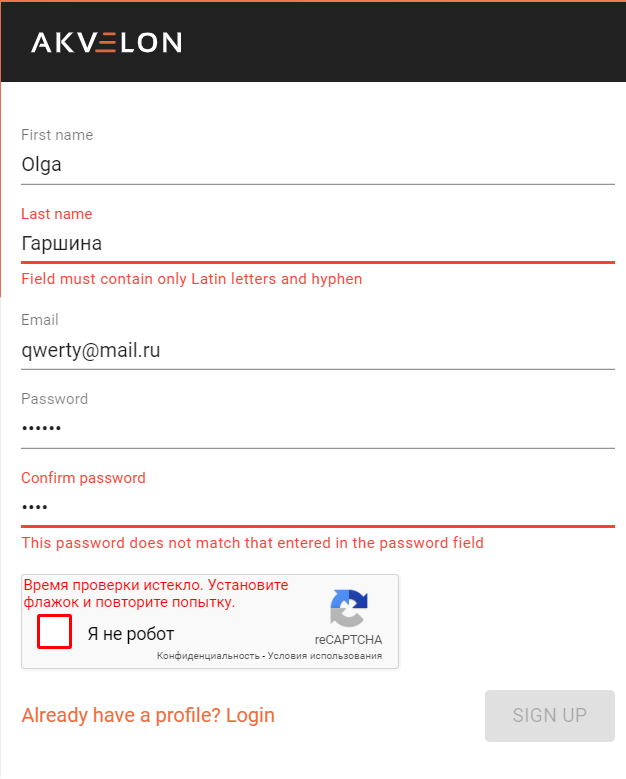
\includegraphics[width=0.7\textwidth]{resources/signup.png}
	\caption{Страница входа на ets.akvelon.com}
	\label{fig:1}
\end{figure}

\section{Сервис уведомлений пользователя, отслеживание прогресса загрузки}

На данном этапе разработки понадобилось оповещать пользователя об ошибках со стороны сервера и другой полезной информации.
Для этого я создала сервис toast.notify и ToastTrigger компонент.

В этом компоненте инициализируются состояния, отвечающие за отслеживание того, отображается плашка с оповещениями или нет, за текст сообщения и за тип уведомления.
При монтировании ToastTrigger как бы говорит toast.notify сервису, что если в коде в каком-нибудь месте вызовется функция-уведомитель
, в параметрах которой будут переданы сообщение и тип уведомления -- состояние
компонента должно поменяться соответственное. На рисунке ~\ref{4} отражен вызов функции в месте кода, где сервер вернул ошибку добавления новой категории.

\begin{figure}[!ht]
	\centering
	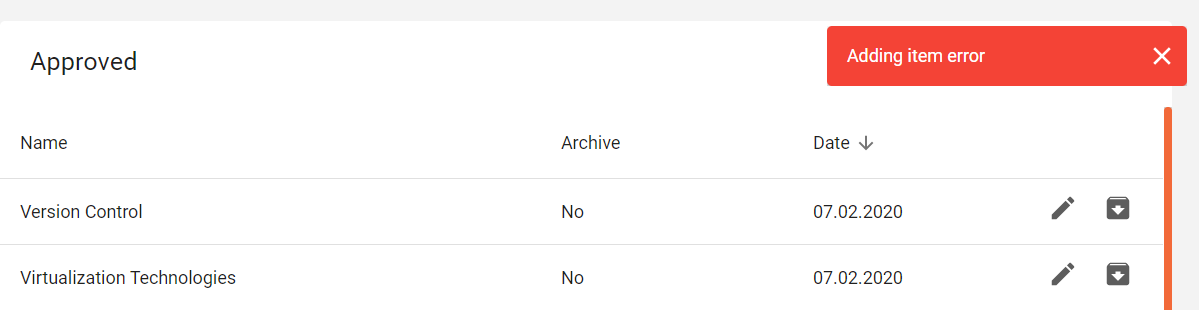
\includegraphics[width=0.9\textwidth]{resources/toasterror.png}
	\caption{Пример уведомления об ошибке}
	\label{4}
\end{figure}

Я поделила оповещения на 4 типа: предупреждение, ошибка, информация и успех. С помощью 
Less очень удобно переопределять стиль плашки в зависимости от параметров, переданных в 
функцию. Вот, например, плашка с информацией, которая вызывается при попытке сохранения резюме, если пользователь 
забыл ввести обязательную информацию (рис. ~\ref{5}).

\begin{figure}[!ht]
	\centering
	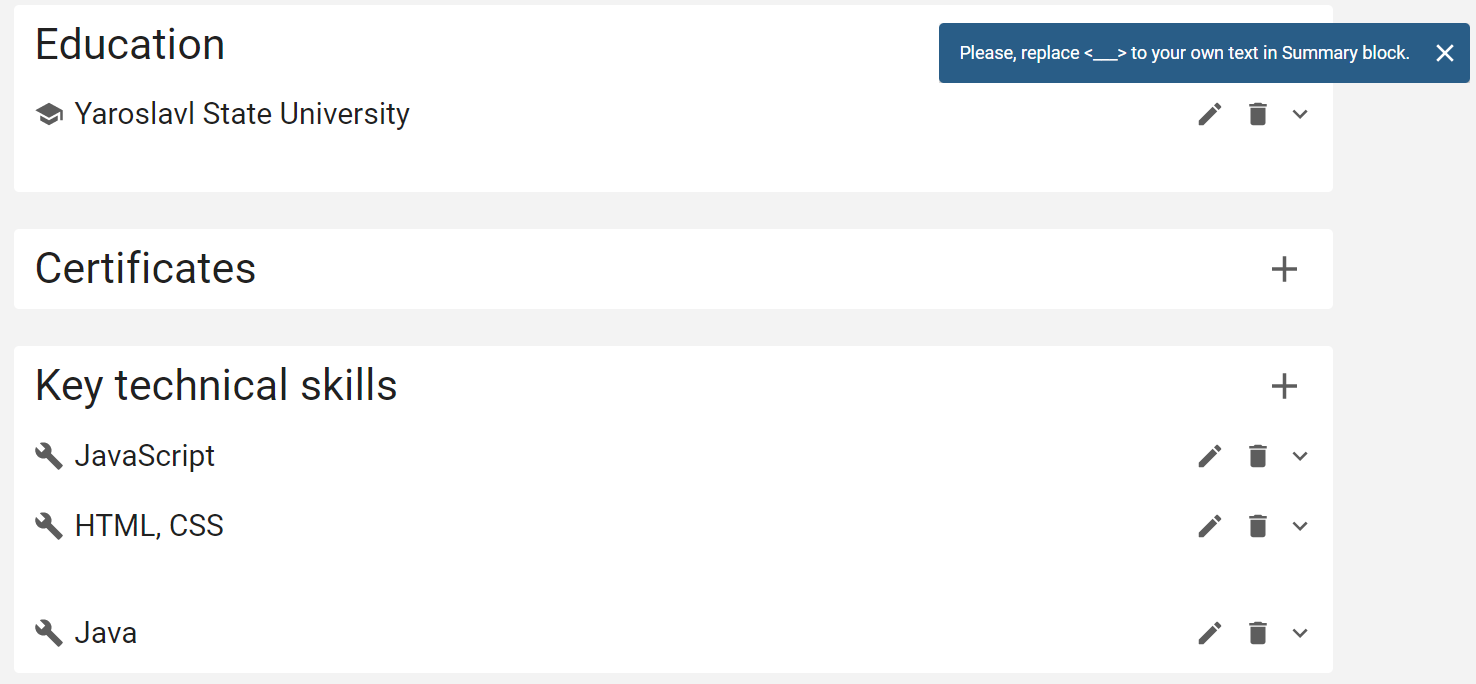
\includegraphics[width=0.9\textwidth]{resources/toast.png}
	\caption{Пример информационного уведомления}
	\label{5}
\end{figure}

Что касается сервиса, показывающего прогресс, то он сделан похоже, за исключением того, что action.notify хранит массив
из подписок на события, которые должны вызывать полосы загрузки. Таким образом на странице может отображаться сразу несколько полос прогресса получения данных в разных местах. Достаточно обернуть их 
компонентом LoaderTrigger, передав имя события, на которое подпишется сервис. 

Данный пример иллюстрирует отображение полос прогресса, пока с сервера подгружаются коллекции компаний и обрабатывается запрос на перенос компании из списка предложенных в список одобренных (рис. ~\ref{6}).
На самом деле это делается мгновенно и полоса прогрузки является больше дружественным интерфейсом для пользователей с медленным инетрнетом. Для отображения прогресса достаточно вызвать две функции: перед началаом асинхронного запроса на сервер, передав параметр "start" и после его окончания, передав "finish".

\begin{figure}[!ht]
	\centering
	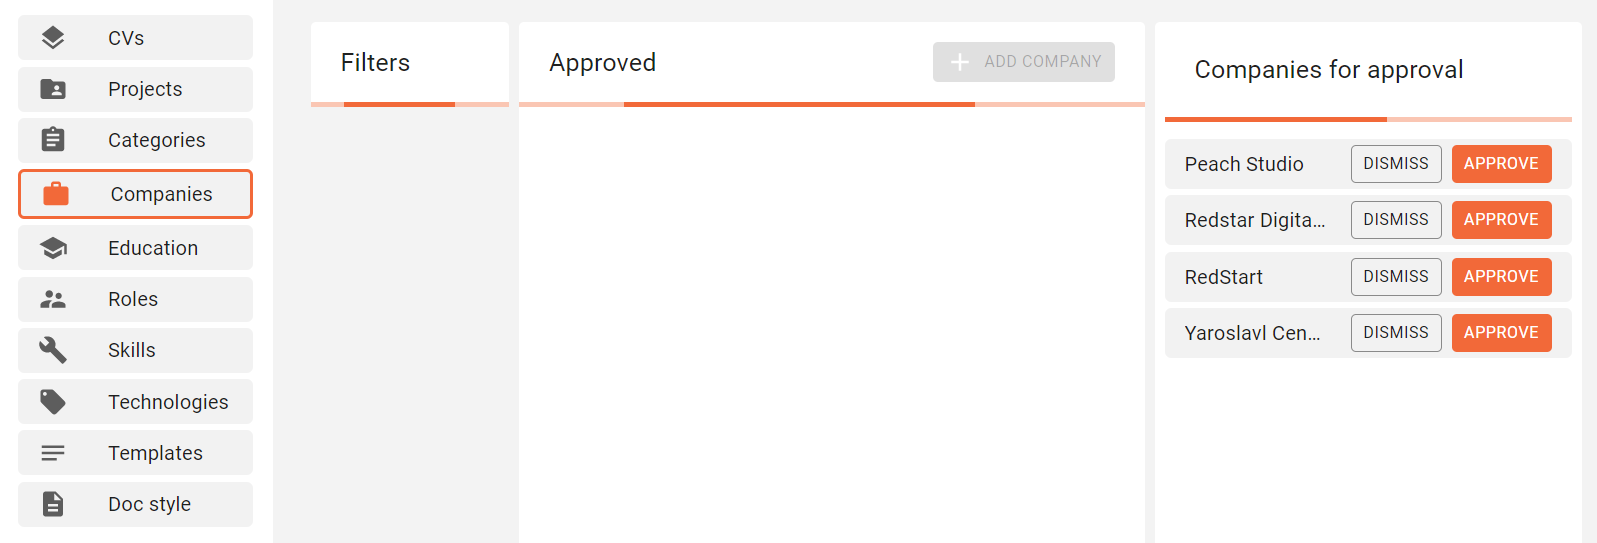
\includegraphics[width=0.9\textwidth]{resources/progress.png}
	\caption{Интерфейс полос загрузки}
	\label{6}
\end{figure}

\section{Страница создания резюме взглядом пользователя}
Создание резюме проходит в несколько этапов и создается для отправки клиенту Аквелона на определенный проект.
Для начала выбирается роль, в зависимости от которой будут подсказываться автоматические предложения для заполнения и сортироваться технологии, которые знает кандидат. Это значит, что тестировщику, например, будет подсказываться текст, 
связанный с написанием UNIT-тестов, а специалисту DevOps - с настройкой CI/CD процессов.

Клиент пожелал, чтобы данные подсказки предлагались в случайном порядке -- это сделает резюме более уникальным, если его будет заполнять не спецаильно обученный рекрутер, а кандидат на позицию.
Далее заполняется поле Summary - краткая выжимка об умениях и качествах работника. В данном поле при нажатии на пункт меню конкретные словосочетания превращаются в шаблоны, выделенные жирным -- такое поведение также попросил заказчик.

Как можно заметить, все это (рис. ~\ref{7}) не похоже на типичное поведение обычного компонента текстового поля из Material UI. Все потому, что данный интерфейс -- это
замаскированный под material design с помощью Less фреймворк Draft.js -- текстовый редактор, переделанный под мои нужды. Было потрачено немало времени, чтобы разобраться в работе библиотеки,
убрать лишние детали и добавить нужные.

\begin{figure}[!ht]
	\centering
	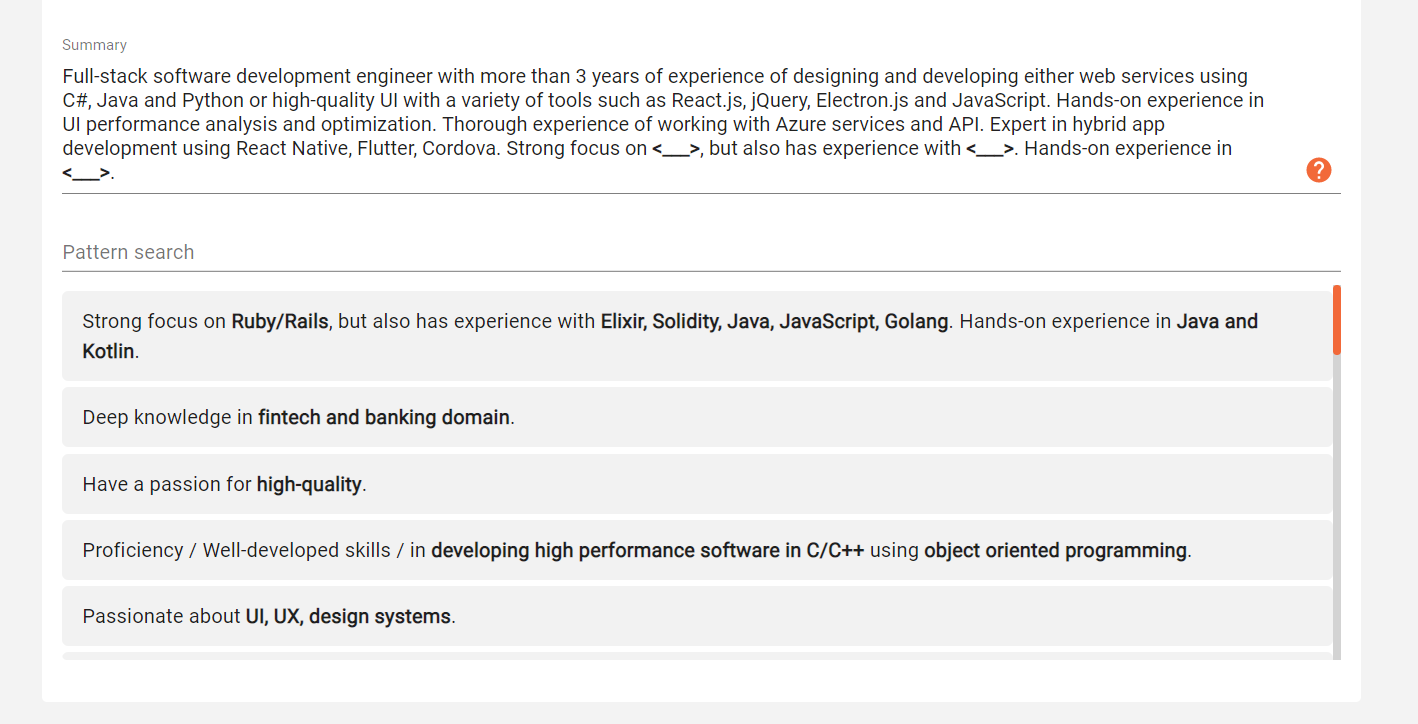
\includegraphics[width=1\textwidth]{resources/summary.png}
	\caption{Интерфейс заполнения поля Summary}
	\label{7}
\end{figure}

Поле роль - созданный мною компонент. Изначально, в Material UI не было достойного решения для выбора пункта из списка, с полем для поиска по нему.
Мне предлагали только сторонние библиотеки, которые имели в себе много лишних зависимостей и много строк кода, которые неприятно читать и сложно в них разбираться.
После чего наступил переломный момент и я решила просто написать свой компонент с тем поведением, который идеально мне подошел. Несмотря на то, что создание простого казалось бы списка со встроенным поискам выглядело простым, 
в процессе написания я столкнулась со многими подводными камнями, связанными с обработкой событий в React. Я искала ответы в интернет сообществах по программированию,
но встречала только некрасивые решения. 

В итоге мне удалось сделать компонент (рис. ~\ref{8}), отвечающий желаемому функционалу и хранящий в состоянии не строку, а целый объект, что
не тратит ресурсы программы на дополнительные преобразования перед отправкой запроса на сервер.

\begin{figure}[!ht]
	\centering
	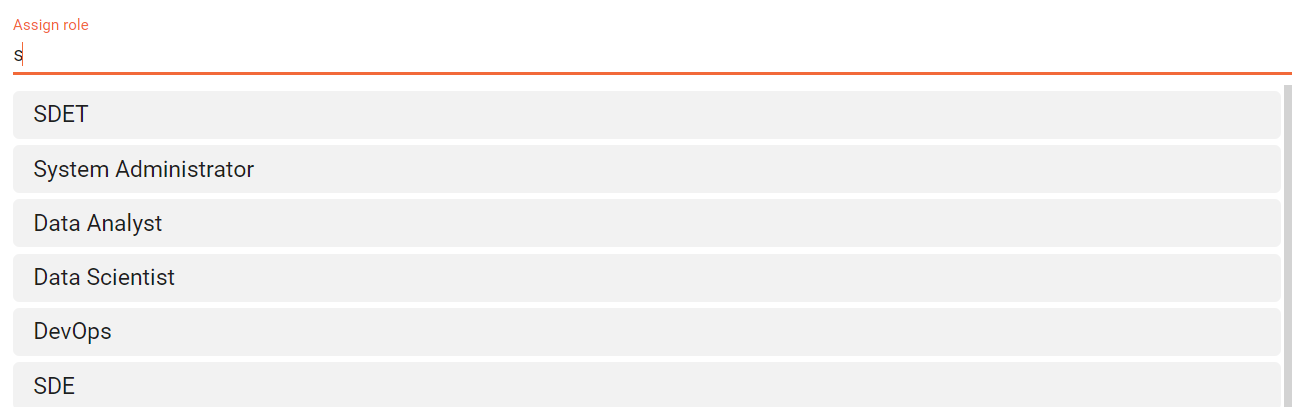
\includegraphics[width=0.8\textwidth]{resources/role.png}
	\caption{Компонент для выбора из списка с поиском}
	\label{8}
\end{figure}

После кандидат заполняет информацию об опыте работы в компаниях в блоке professional expirience. Я вдохновлялась дизайном заполнения информации на сайте linkedin при разработке данного блока (рис. ~\ref{9}).
На его примере я хочу показать функционал подсказок для автозаполнения и принцип пополнения базы данных.
\begin{figure}[!ht]
	\centering
	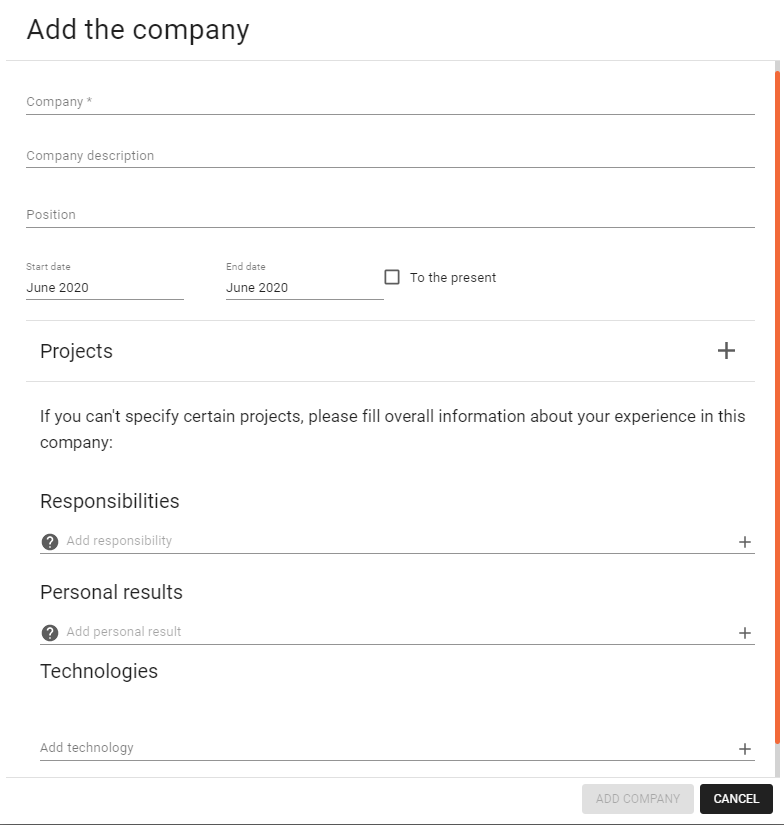
\includegraphics[width=1\textwidth]{resources/companycard.png}
	\caption{Диалоговое окло добавления компании}
	\label{9}
\end{figure}

Как только пользователь начинает набирать текст в поле Company, под ним раскрывается список тех компаний для заполнения, которые включают в себя набранное буквосочетание.
Если база не включает в себя название компании, которое хочет вбить кандидат, то после нажатия кнокпи "Add" она
отправляется на рассмотрение админами в часть интерфейса, скрытого от обычного пользователя.

Далее идут обычные текстовые поля для заполнения крадкой сводки о компании и о занимаемой позиции в ней.

После кандидату необходимо указать время работы в компании. При нажатии на на поля start date/end date поочередно открывается интерфейс для выбора года и месяца (рис. ~\ref{10}). 
В случае, если кандидат все еще является сотрудником описываемой компании, он может нажать галочку рядом с "To the present", тем самым автоматически скроется возможность выбора даты окончания работы.

\begin{figure}[!ht]
	\centering
	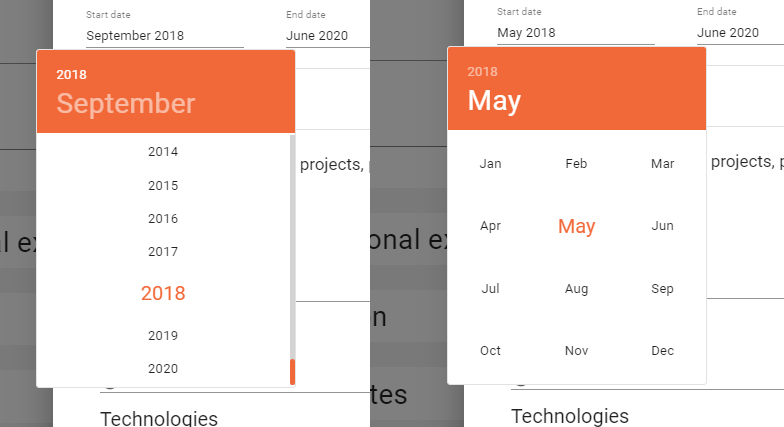
\includegraphics[width=1\textwidth]{resources/dates.png}
	\caption{Интерфейс выбора даты}
	\label{10}
\end{figure}

Потом подразумевается заполнение информации о проектах. Если кандидат не может выделить каких-то конкретных, то требуется заполнить общую информацию. Предлагается внести данные о персональных результатах, выполненных задачах и используемых технологиях.
Некоторые люди стакиваются с проблемой того, чо они не могут сразу быстро вспомнить все свои достижения.
Для этого я добавила возможность раскрыть по кнопке со знаком вопроса меню с подсказками шаблонных фраз, которые как и в поле Summary относятся к выбранной в начале роли. Если кандидат оставил место для шаблона незаполненным -- это валидируется.
Описанный выше функционал можно наблюдать на рисунке ~\ref{11}.

\begin{figure}[!ht]
	\centering
	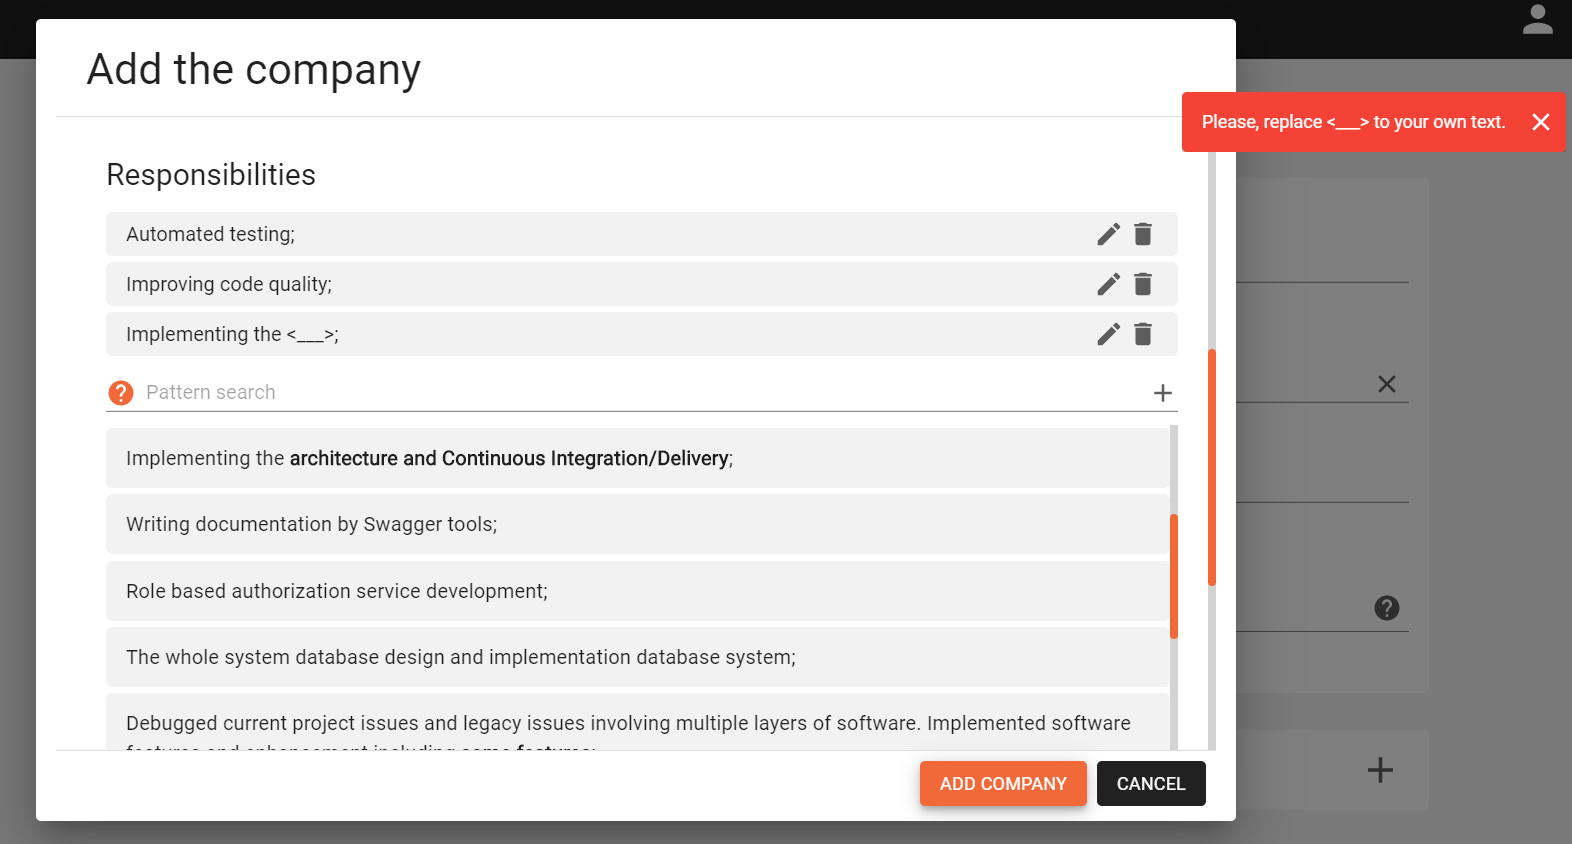
\includegraphics[width=1\textwidth]{resources/responsibility.png}
	\caption{Интерфейс заполнения информацией поля responsibility и её валидация}
	\label{11}
\end{figure}

Заполнение блока заканчивается указанием используемых в компании технологий, которые автозаполняются и попадают в базу данных на рассмотрение админами.
Так как технологии являются коллекцией с самой большой базой, их модерация достойна отдельного внимания. Чтобы глаз рекрутера мог зацепиться за потенциальное некорректное слово, я 
сделала цветовой акцент на интерфейсе. Таким образом, одобренные технологии окрашены в оранжевый, а остальные в серый (рис. ~\ref{12}). Чтобы пользователь не засорял базу альтернативными названиями технологий было решено привязывать к ним список синонимов. Так, введя в поле JS и нажав ввод,
кандидат получит корректное названия языка на выходе -- JavaScript.

\begin{figure}[!ht]
	\centering
	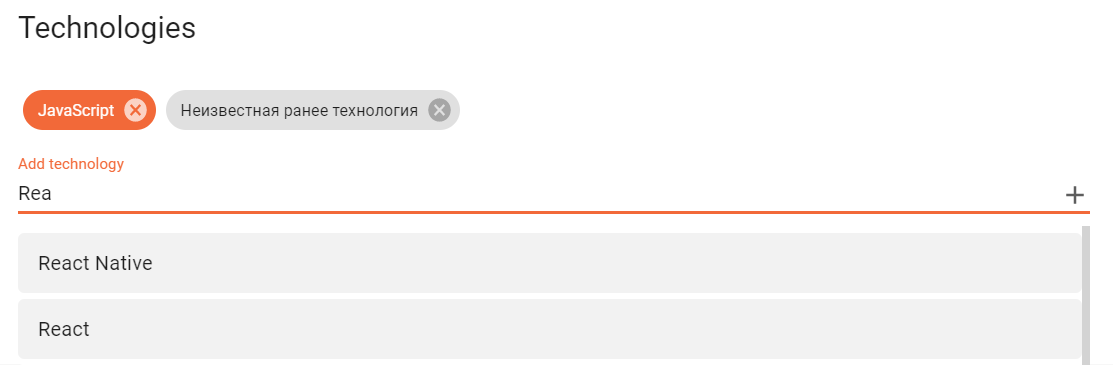
\includegraphics[width=1\textwidth]{resources/technologies.png}
	\caption{Заполнение инфо-блока технологиями}
	\label{12}
\end{figure}

Если же проекты к заполнению все же есть, то по нажатию на плюс всплывает еще одно диалоговое окно, где нужно
указать название проекта, его описание и те же пункты, что и в блоке добавления после выбора времени работы на позиции.

Всё доступно для редактирования и полного удаления, все информационные списки можно сворачивать и разворачивать. Чтобы ненужная на момент заполнения информация не мешала на фоне в развернутом состоянии, в режиме редактирования сиви находится 
только один логический блок.

Преимущество данного UX-решения особенно хорошо наблдается в режиме просмотра резюме. В нем можно развернуть всю структуру документа для полноты восприятия, страница приложения станет действительно длинной (рис. ~\ref{13}), особенно если речь идет о опыте работа программиста-сеньора.
Также в данном режиме полностью отсутствуют отвлекающие кнопки для какого-либо взаимодействия, он отлично подходит для того, чтобы рекрутер мог просто поделиться ссылкой на страницу с голой информацией о резюме.

Блоки education, certificates и key technical skills по своей структуре похожи на блок professional expirience, а вот technical summary хочется уделить особое внимание.
В нем автоматически сгенерирован и категоризирован список всех технологий, который пользователь затрагивал, заполняя резюме. Блок меняет свой вид при изменении роли, потому что у программиста с большим стеком он
громаден, а клиент хочет сэкономить свое время и увидеть приоритетную для него информацию в первых же строках. Если технологию указывалю в резюме на различных проектах и различных компаниях, написанный мною алгоритм валадирует хранение в данном списке только уникальных наименований технологий.


Также это то место, где кандидат может вбить изученные им вне работы технологии. Иногда бывало, что это тоже играло роль, когда клиенты Akvelon-а выбирали, на какой стек поставить работника на проекте.

Технологии, категории которых не определены, всегда попадают в Others по регламенту стандартного Akvelon-резюме. Список категорий у каждой роли свой и фиксирован, поэтому если кандидат не знает ни одной технологии из категории, ее строка остается пустой (рис. ~\ref{14}).
\begin{figure}[!ht]
	\centering
	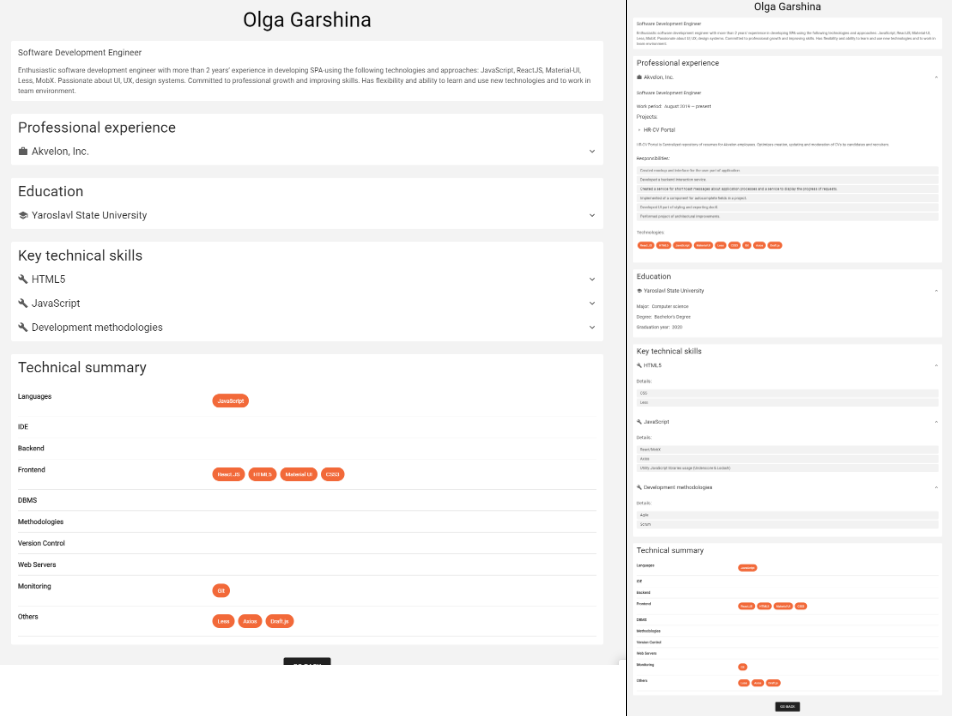
\includegraphics[width=1\textwidth]{resources/expand.png}
	\caption{Слева отображен режим просмотра с примером со свернутыми инфо-блоками, справа с развернутыми}
	\label{13}
\end{figure}
\begin{figure}[!ht]
	\centering
	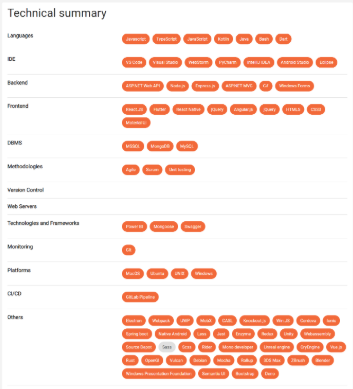
\includegraphics[width=1\textwidth]{resources/tecsummary.png}
	\caption{Блок technical summary одного из работников Akvelon}
	\label{14}
\end{figure}
\section{Таблица всех резюме взглядом пользователя}

Для удобства поиска резюме и фильтрации была реализована идея с таблицей (рис. ~\ref{15}). Фильтрацию можно воспроизводить по имени, роли, позиции,
проекту, по дате и по типу резюме исходя из того, скрыт он от глаз или нет. В зависимости от нужд пользователя, количество строк в таблице можно менять от 5 до 50 на странице.
Нажимая на кнопку с троеточием кандидат может заархивировать (спрятать) резюме, копировать, перейти в режим редактирования или просмотра, а также экспортировать
стилизованный документ в формате .docx. Пользователь может знать информацию о проекте, к которому привязано его резюме, но не может изменить ее, так как эта привелегия рекрутеров, которые подразумеваются
администраторами сайта.

\begin{figure}[!ht]
	\centering
	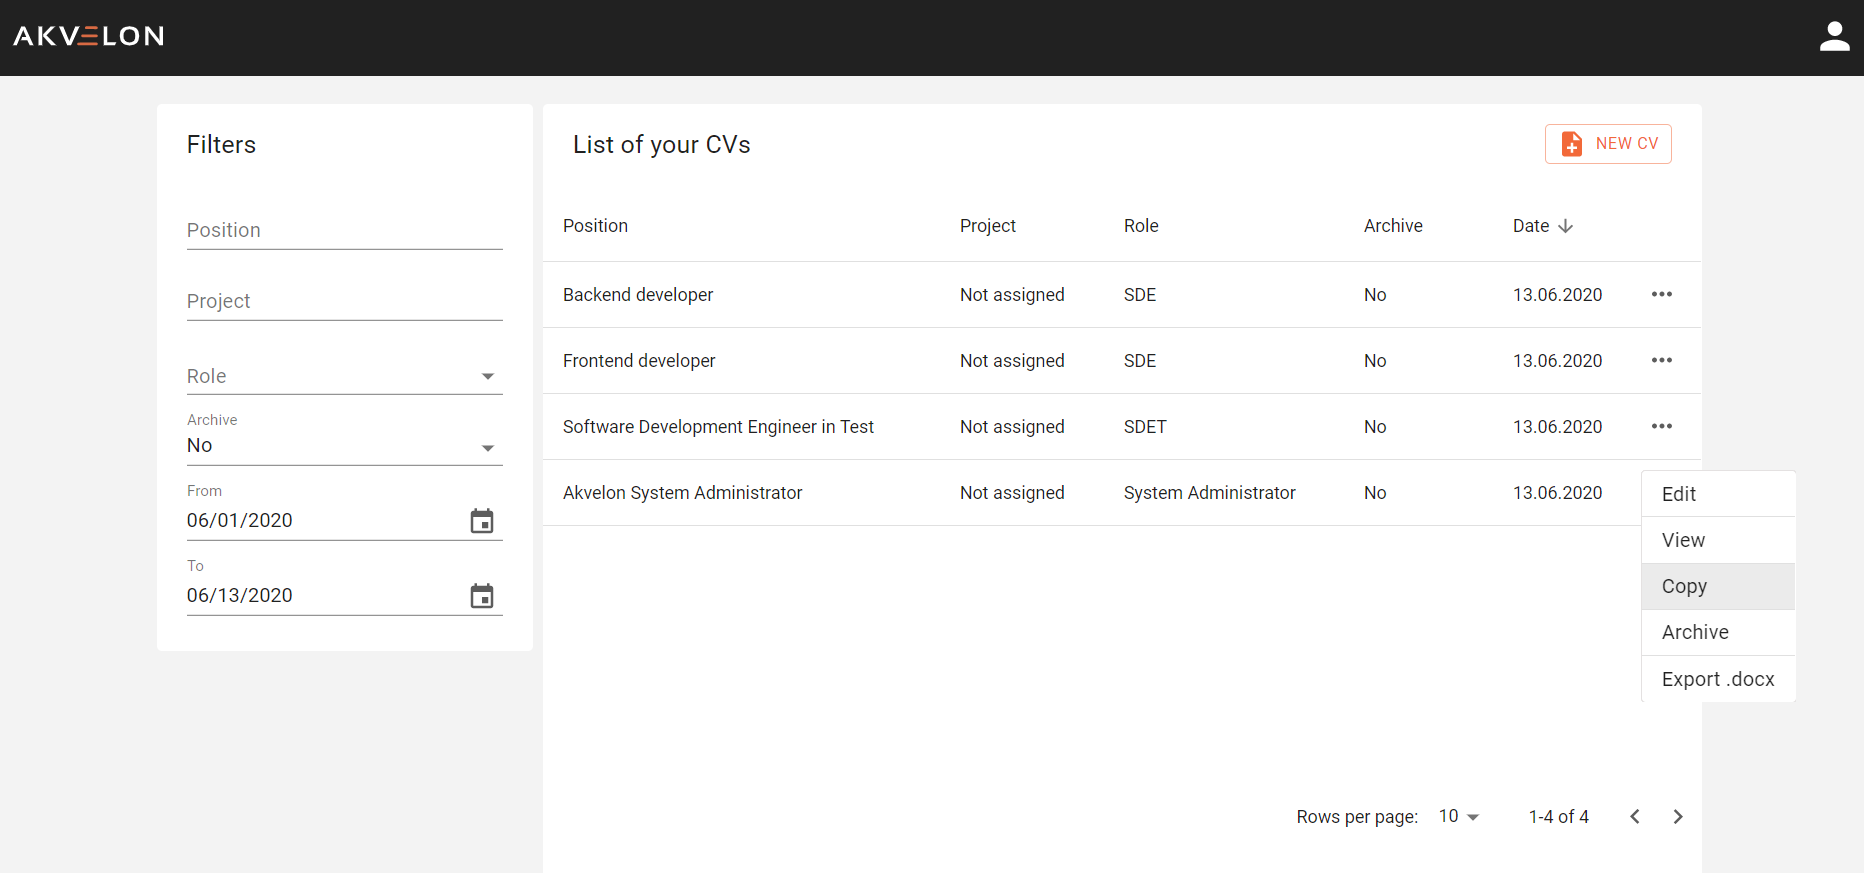
\includegraphics[width=1\textwidth]{resources/cvlistuser.png}
	\caption{Таблица со списком пользовательских резюме}
	\label{15}
\end{figure}

\section{Отладка умных контрактов}

\section{Визуальный интерфейс для взаимодействия с развернутыми умными контрактами}

\chapter{Результаты решения задачи}

В результате решения задачи было получено расширение для VSCode

\chapternonum{Заключение}

% Если нужно, меняем название Литература
\renewcommand{\bibname}{Список литературы} 
\begin{thebibliography}{9}
% Если нужно сделать N. вместо [N] 
% \makeatletter\renewcommand{\@biblabel}[1]{#1.}\makeatother

\bibitem{VSCode}
Visual Studio Code - Code Editing. Redefined
URL: https://code.visualstudio.com
(дата доступа: 09.06.2020)

\end{thebibliography}

\end{document}
